

\chapter{Analisi Sintattica}
$S \rightarrow cAd$
$A \rightarrow ab | a$

%%%%%%%%%%%%%%%%%%%%%%%%%%%%%%%%%%%%%%%%%%%%%%%%%%%%%%%%%%%%%%%%%%%%%%%%%%%%%%%%%%%%%%%%%%%%%%%%
\section{Parsing Top-down}
Parto dal starting symbol ed espando le derivazioni dando priorit\'a alle derivazioni pi\'u a sinistra.
Cerco quindi di ricostruire una derivazione leftmost della stringa w data in input.

$w\$, \$ \not\in V$\\
$w=cabd$

Per ricostruire la parola w parto dalla prima derivazioine $S \rightarrow cAd$ derivo la A pi\'u a sinistra (leftmost) e posso scegliere 
fra $a$ ed $ab$; scelgo $a$ e mi accorgo che ho sbagliato, torno in dietro e scelgo $ab$.

%%%%%%%%%%%%%%%%%%%%%%%%%%%%%%%%%%%%%%%%%%%%%%%%%%%%%%%%%%%%%%%%%%%%%%%%%%%%%%%%%%%%%%%%%%%%%%%%
\section{Parsing Top-down predittivo (o non ricorsivo)}
Cambio la grammatica sopra in: 
$S \rightarrow cAd$
$A \rightarrow aB$
$B \rightarrow b | \varepsilon $
Cos\'i non sbaglio 

%%%%%%%%%%%%%%%%%%%%%%%%%%%%%%%%%%%%%%%%%%%%%%%%%%%%%%%%%%%%%%%%%%%%%%%%%%%%%%%%%%%%%%%%%%%%%%%%
\subsection{Grammatica LL(1)}
prima L: leggiamo la input string da sinistra\\
seconda L: ricostruiamo una leftmost derivazione\\
(1): decidiamo quale operazione effettuare guardando un solo simbolo in input\\
Le grammatiche LL(1) sono un subset delle grammatiche libere.

\section{Algoritmi di Parsing}
\begin{tabular}{lc}
    input buffer    &   w$\$$   \\
    stack           &   bottom[$ \$ \qquad $] top \\
    parsing table   & con tante righe quante non terminali, tante colonne quante terminali ($ \$ $ incluso)\\
                    & in ogni cella metto un'eventuale trasformazione o \lq\lq error \rq\rq \\
\end{tabular}

%%%%%%%%%%%%%%%%%%%%%%%%%%%%%%%%%%%%%%%%%%%%%%%%%%%%%%%%%%%%%%%%%%%%%%%%%%%%%%%%%%%%%%%%%%%%%%%%
\subsection{Algoritmo di parsing non-ricorsivo}
\begin{center}
    \begin{tabular}{ll}
        input   &   stringa w, tabella parsing non ricorsivo T, per G\\
        output  &   derivazione leftmost di w se $w \in L(G)$, error() altrimenti\\
    \end{tabular}
\end{center}

\begin{lstlisting}
    //init
    buffer = {w$};
    stack.push($S);

    let b il primo simbolo di w 
    let x il top dello stack 

    while(x != $){
        if(x == b){
            pop(x);
            let b il simbolo necessario di w;
        } else if(x e'' terminale){
            error();
        } else if(T[x,b] contiene X -> Y1...Yn){
            return X -> Y1...Yn;
            pop(x);
            push(Yn...Y1)
        }
        let x il top dello stack
    }
\end{lstlisting}

%%%%%%%%%%%%%%%%%%%%%%%%%%%%%%%%%%%%%%%%%%%%%%%%%%%%%%%%%%%%%%%%%%%%%%%%%%%%%%%%%%%%%%%%%%%%%%%%%%%%%%%%%
\subsection{Esempio}
$E \rightarrow TE'$ \\
$E' \rightarrow +TE'|\varepsilon$\\
$T \rightarrow FT'$\\
$T' \rightarrow *FT'|\varepsilon$\\
$F \rightarrow id$\\

\begin{tabular}{|c|c|c|c|c|}
    \hline
            &   id                      &   +                           &   *   &   $\$$    \\
    \hline
        E   &   $E \rightarrow TE'$     &                               &     &      \\
    \hline
        E'  &                           &   $E' \rightarrow TE'$        &     &   $E' \rightarrow \varepsilon $    \\
    \hline
        T   &   $T \rightarrow FT'$     &                               &      &      \\
    \hline
        T'  &                           &   $T' \rightarrow \varepsilon$    &   $T' \rightarrow *FT'$   &   $T' \rightarrow \varepsilon$    \\
    \hline
        F   &   $F \rightarrow id$      &                               &      &       \\
    \hline
\end{tabular}

\begin{tabular}{|c|c|c|}
    \hline
    pila & input & output \\
    \hline
    $\$ $\underline{E}  &   \underline{id}+id*id$ \$ $  &   $E \rightarrow TE'$ \\
    \hline
    $\$ $ E \underline{T'}  &   &   $E \rightarrow TE' $ \\
    \hline
    $\$ ET'$\underline{F}  &   &   $F \rightarrow id $ \\
    \hline
    $\$ $ ET' \underline{id}  &    &   \\
    \hline
    $\$ E'$\underline{T''}  &  +\underline{id}*id $\$$  &   $T'' \rightarrow \varepsilon $ \\
    \hline
    $\$ $\underline{E'}  &    &   $E' \rightarrow TE'$ \\
    \hline
    $\$ $ E'T \underline{+}  &   \underline{id}*id$ \$ $  &   \\
    \hline
    $\$ $ E'\underline{T}  &     &   \\
    \hline
        &     ...Avanti cos\i     &   \\
    \hline
\end{tabular}

\Tree[.E [.T [.F id ] [.T' $\varepsilon$ ] ] [.E' + [.T  [.F id ] [.T' * [.F id ] [.T' $\varepsilon$ ] ] ] [.E' $\varepsilon$ ] ] ]

%%%%%%%%%%%%%%%%%%%%%%%%%%%%%%%%%%%%%%%%%%%%%%%%%%%%%%%%%%%%%%%%%%%%%%%%%%%%%%%%%%%%%%%%%%%%%%%%
\subsection{Esercizio}
$S \rightarrow aA | bB$\\
$A \rightarrow c $\\
$B \rightarrow d $\\

$w = ac\$ $ \\

Parsing: $S \implies aA \implies ac $\\

Nella tabella metto le produzioni della grammatica:

\begin{tabular}{|l|l|l|l|l|l|}
        &   a   &   b   &   c   &   d   &   $\$$    \\
    S   &   $S \rightarrow aA$   &    $S \rightarrow bB$   &      &      &      \\
    A   &      &      &  $A \rightarrow c$     &      &      \\
    B   &      &      &       &  $B \rightarrow d$    &      \\  
\end{tabular}

%%%%%%%%%%%%%%%%%%%%%%%%%%%%%%%%%%%%%%%%%%%%%%%%%%%%%%%%%%%%%%%%%%%%%%%%%%%%%%%%%%%%%%%%%%%%%%%%
\section{Calcolo First}
Data una generica $\alpha \in V^*$ per G=(V, T, S, P), first($\alpha$) \'e l'insieme dei simboli terminali b tali che $\alpha \implies bv$.
Inoltre se $\alpha \implies \varepsilon $ allora $\varepsilon \in first(\alpha )$

%%%%%%%%%%%%%%%%%%%%%%%%%%%%%%%%%%%%%%%%%%%%%%%%%%%%%%%%%%%%%%%%%%%%%%%%%%%%%%%%%%%%%%%%%%%%%%%%
\subsection{Esercizio}
$S \rightarrow A|B$\\
$A \rightarrow a|C$\\
$C \rightarrow \varepsilon$\\
Allora first(A) = $\{ a, \varepsilon \}$ ($\varepsilon$ perch\'e posso fare $A \implies C \implies \varepsilon $). 

%%%%%%%%%%%%%%%%%%%%%%%%%%%%%%%%%%%%%%%%%%%%%%%%%%%%%%%%%%%%%%%%%%%%%%%%%%%%%%%%%%%%%%%%%%%%%%%%
\subsection{Esercizio}
$S \rightarrow A|B$\\
$A \rightarrow a|C$\\
$C \rightarrow bB$\\
Allora first(A) = $\{ a, b \}$ (b perch\'e posso fare $A \implies C \implies bB$, ma B non esiste). 

%%%%%%%%%%%%%%%%%%%%%%%%%%%%%%%%%%%%%%%%%%%%%%%%%%%%%%%%%%%%%%%%%%%%%%%%%%%%%%%%%%%%%%%%%%%%%%%%
\subsection{Esercizio}
$S \rightarrow A|B$\\
$A \rightarrow a|C$\\
$C \rightarrow bB$\\
$B \rightarrow c$\\
Allora first(A) = $\{ a, b \}$ ($A \implies C \implies bB \implies bc$, ma tengo solo il primo simbolo (b)) 

%%%%%%%%%%%%%%%%%%%%%%%%%%%%%%%%%%%%%%%%%%%%%%%%%%%%%%%%%%%%%%%%%%%%%%%%%%%%%%%%%%%%%%%%%%%%%%%%
\subsection{Esercizio}
$A \rightarrow A|C$\\
$C \rightarrow bB|\varepsilon$\\
$B \rightarrow c$\\
Allora first(A) = $\{ a, b, \varepsilon\}$

G=(V,T,S,P)
Sia $X \in V$. L'insieme first(X) viene calcolato come segue:
\begin{itemize}
    \item[1)] inizializzo first(X) vuoto $\forall\ X \in V$\\
    \item[2)] se $X \in T$ allora first(X) = $\{ X \}$\\
    \item[3)] se $X \rightarrow \varepsilon \in P$ allora aggiungere $\varepsilon$ ai first(X)\\
    \item[4)] se $X \rightarrow Y_1...Y_n \in P$, con $n \geq 1$ allora uso la seguente procedura:\\
\end{itemize}
\begin{lstlisting}
    j = 1;
    while(j <= n){
        aggiungere ai first(X) ogni b tale che b in first(Yj)
        if(epsilon in first(Yj)){
            j++;
        } else {
            break;
        }
    }

    if(j == n+1){
        aggiungere epsilon ai first(X);
    }
\end{lstlisting}

Sia $\alpha=Y_1 ... Y_n,\ n\geq 1$, allora first($\alpha$) \'e calcolato sotituendo a X alpha:
\begin{lstlisting}
    j = 1;
    while(j <= n){
        aggiungere ai first(alpha) ogni b tale che b in first(Yj)
        if(epsilon in first(Yj)){
            j++;
        } else {
            break;
        }
    }

    if(j == n+1){
        aggiungere epsilon ai first(alpha);
    }
\end{lstlisting}

%%%%%%%%%%%%%%%%%%%%%%%%%%%%%%%%%%%%%%%%%%%%%%%%%%%%%%%%%%%%%%%%%%%%%%%%%%%%%%%%%%%%%%%%%%%%%%%%%%%%%%%
\subsection{Esercizio}
$E \rightarrow T E'$\\
$E' \rightarrow +T E' | \varepsilon $\\
$T \rightarrow FT'$\\
$T' \rightarrow *FT'| \varepsilon $\\
$F \rightarrow (E)|id $\\

First:
$E = \{ id, ( \}$ ovviamente ha gli stessi first di T per $E \rightarrow T E'$\\
$E' = \{ +, \varepsilon \}$\\
$T = \{ id, ( \}$ ha gli stessi first di F per $T \rightarrow FT'$\\
$T' = \{ *, \varepsilon \}$\\
$F = \{ id, ( \}$\\

Per generare id + id: \Tree[.E [.T [.F id ] [.T' $\varepsilon$ ] ] [.E' + [.T [.F id ] [.T' $\varepsilon$ ] ] [.E' $\varepsilon$ ] ] ]\\

Mancano le parentesi fra i terminali nella tabella...
\begin{tabular}{|c|c|c|c|c|}
    \hline  
        &   id                              &   +   &   *   &   $\$$    \\
    \hline  
    E   &   $E \rightarrow T E'$            &       &       &   \\
    \hline  
    E   &   &   $E' \rightarrow T E'$       &       &   $E' \rightarrow \varepsilon $ \\
    \hline       
    T   &   $T \rightarrow FT'$             &       &       &   \\     
    \hline   
    T'  &   &  $T' \rightarrow \varepsilon $   &   $T' \rightarrow *FT'$    & $T' \rightarrow \varepsilon $  \\   
    \hline    
    F   &   $F \rightarrow id $             &       &       &   \\    
    \hline  
\end{tabular}

%%%%%%%%%%%%%%%%%%%%%%%%%%%%%%%%%%%%%%%%%%%%%%%%%%%%%%%%%%%%%%%%%%%%%%%%%%%%%%%%%%%%%%%
\section{Follow}
$\forall\ A \in V \backslash T, $ follow(A):
\begin{lstlisting}
    follow(A) = emptySet per ogni A in (V \ T);
    follow(S).push($);

    repeat{
        foreach(B -> alpha A beta in P){
            if(beta == epsilon){
                follow(A).push(follow(B));
            } else {
                follow(A).push(first(beta) \ epsilon);
                if(epsilon in first(beta)){
                    follow(A).push(follow(B));
                }
            }
        }
    } until (saturazione);
\end{lstlisting}

%%%%%%%%%%%%%%%%%%%%%%%%%%%%%%%%%%%%%%%%%%%%%%%%%%%%%%%%%%%%%%%%%%%%%%%%%%%%%%%%%%%%%%%
\subsection{Esempio}

$S \rightarrow aABb$\\
$A \rightarrow Ac|d$\\
$B \rightarrow CD$\\
$C \rightarrow e|\varepsilon$\\
$D \rightarrow f|\varepsilon$\\

\begin{tabular}{ccc}
              &   First                     &   Follow      \\    
    $S=$      &    $\{ a \}$                &   $\{ \$ \}$        \\
    $A=$      &    $\{ d \}$                &   $\{e,f,b$ (da $S \rightarrow aABb$), c (da $A \rightarrow Ac$)$\}$ \\
    $B=$      &    $\{ e,f,\varepsilon \}$     &   $\{b \text{ (da } S \rightarrow aABb)\}$   \\
    $C=$      &    $\{ a,\varepsilon \}$       &   $\{f \text{ (da } B \rightarrow CD)\}$      \\
    $D=$      &    $\{ f,\varepsilon \}$       &   $\{\}$      \\
\end{tabular}

%%%%%%%%%%%%%%%%%%%%%%%%%%%%%%%%%%%%%%%%%%%%%%%%%%%%%%%%%%%%%%%%%%%%%%%%%%%%%%%%%%%%%%%
\subsection{Esempio}

$S \rightarrow aA|aBc$\\
$A \rightarrow Bd|Cc$\\
$B \rightarrow e|\varepsilon$\\
$C \rightarrow f|\varepsilon$\\

\begin{tabular}{ccc}
              &   First                   &   Follow            \\    
    $S=$      &    $\{ a, b \}$           &   $\{ \$ \}$        \\
    $A=$      &    $\{ e,d,f,c \}$        &   $\{ \$,(?) \}$    \\
    $B=$      &    $\{ e,\varepsilon \}$     &   $\{ c,d \}$       \\
    $C=$      &    $\{ f,\varepsilon \}$     &   $\{ c \} $        \\
\end{tabular}

%%%%%%%%%%%%%%%%%%%%%%%%%%%%%%%%%%%%%%%%%%%%%%%%%%%%%%%%%%%%%%%%%%%%%%%%%%%%%%%%%%%%%%%
\subsection{Esempio}

$E \rightarrow TE'$\\
$E' \rightarrow +TE'|\varepsilon$\\
$T \rightarrow FT'$\\
$T' \rightarrow *FT'|\varepsilon$\\
$F \rightarrow (E)|id $\\

\begin{tabular}{cccc}
              &   First                     &   Follow      &                               \\    
    $E=$      &    $\{ id, ( \}$            &   $\{\$,)\}$  &                               \\
    $E'=$     &    $\{ +, \varepsilon \}$      &   $\{\}$      &   ed eredita i follow di E    \\
    $T=$      &    $\{ id, ( \}$            &   $\{+\}$     &   ed eredita i follow di E,E' \\
    $T'=$     &    $\{ +, \varepsilon \}$      &   $\{\}$      &   ed eredita i follow di T    \\    
    $F=$      &    $\{ id, ( \}$            &   $\{*\}$     &   ed eredita i follow di T, T'\\
    & & Quindi diventa: & \\
    $E=$      &    $\{ id, ( \}$            &   $\{\$,)\}$      &   \\
    $E'=$     &    $\{ +, \varepsilon \}$      &   $\{\$,)\}$      &   \\
    $T=$      &    $\{ id, ( \}$            &   $\{+, \$\}$     &   \\
    $T'=$     &    $\{ +, \varepsilon \}$      &   $\{+, \$\}$     &   \\    
    $F=$      &    $\{ id, ( \}$            &   $\{*, +, \$\}$  &   \\
\end{tabular}

Parsing di \lq\lq$id+id*id\$$\rq\rq\ $E \rightarrow TE' \rightarrow FT'E' \rightarrow idT'E' \rightarrow ...$ 

%%%%%%%%%%%%%%%%%%%%%%%%%%%%%%%%%%%%%%%%%%%%%%%%%%%%%%%%%%%%%%%%%%%%%%%%%%%%%%%%%%%%%%%%%%%%%%%%%%%%%%%%%%%%
\section{Costruzione delle tabelle di parsing predittivo top-down}
\begin{center}
    \begin{tabular}{ll}
        input   &   G=(V,T,S,P) \\
        output  &   Tabella T di parsing predittivo top-down se G \'e LL(1)\\
    \end{tabular}
\end{center}

\begin{lstlisting}
    foreach((A -> alpha) in P){
        forall b in first(alpha), poniamo A -> alpha in T[A, b];
        if(epsilon in first(alpha)){
            forall x in follow(A) poniamo A -> alpha in T[A, x];
        }
    }
    
    poniamo error() in tutte le entry di T che sono rimaste vuote;

    if(la tabella non ha entry multiply-defined)
        G e'' LL(1);

\end{lstlisting}

%%%%%%%%%%%%%%%%%%%%%%%%%%%%%%%%%%%%%%%%%%%%%%%%%%%%%%%%%%%%%%%%%%%%%%%%%%%%%%%%%%%%%%%
\subsection{Esempio}

$E \rightarrow E+T|T $\\
$T \rightarrow T*F|T $\\
$F \rightarrow (E)|id $\\

\begin{tabular}{cccc}
              &   First                    &   Follow                               &                           \\    
    $E=$      &    $\{ ( id \}$            &   $\{ \$, +, ) \}$                     &   $\{ \$, +, ) \}$        \\
    $T=$      &    $\{ ( id \}$            &   $\{ * \}$ ed eredita i follow di E   &   $\{ \$, +, *, ) \}$     \\
    $F=$      &    $\{ ( id \}$            &   $\{ \}$ ed eredita i follow di T     &   $\{ \$, +, *, ) \}$     \\
\end{tabular}
Guardo se \'e LL(1)

\begin{tabular}{|l|l|}
    \hline
        &   id  \\
    \hline
    E   &   $E \rightarrow E + T $  \\
        &   $E \rightarrow T $      \\
    \hline
\end{tabular}
Pur non sviluppando tutta la tabella si vede che ci sono entry multiple quindi non \'e LL(1).

Una grammatica G esibisce \textbf{left recursion} se per qualche $A \in V \backslash T$ e per qualche $\alpha \in V^*,\ A \rightarrow ^* A\alpha $.

La left recursion \'e immediata se G ha almeno una produzione del tipo $A \rightarrow a \alpha$ (ovvero se succede nel passato).
Nell'esempio di prima c'era left recursion immediata nei primi due casi ($E \rightarrow E\alpha \land T \rightarrow T\alpha $).

\begin{tcolorbox}\begin{center}
    Proposizione: ogni grammaticha che esibisce left recursion non \'e LL(1).
\end{center}\end{tcolorbox}

$A \rightarrow B$\\
$B \rightarrow Aa$\\
Esempio di left recursion in pi\'u passi.

%%%%%%%%%%%%%%%%%%%%%%%%%%%%%%%%%%%%%%%%%%%%%%%%%%%%%%%%%%%%%%%%%%%%%%%%%%%%%%%%%%%%%%%%%%%%%%%%%%
\section{Eliminazione Left Recursion immediata}

%%%%%%%%%%%%%%%%%%%%%%%%%%%%%%%%%%%%%%%%%%%%%%%%%%%%%%%%%%%%%%%%%%%%%%%%%%%%%%%%%%%%%%%%%%%%%%%%%%
\subsection{Esempio}
$A \rightarrow A \alpha | \beta $, con $\beta != A \land \alpha != \varepsilon$ diventa:\\
$A \rightarrow \beta A'$\\
$A' \rightarrow \alpha A' | \varepsilon$\\

Pi\'u in generale
$A \rightarrow A\alpha _1 | ... | A\alpha _n | \beta _1 | ... | \beta _n $, $\beta _1, ..., \beta _n != A_y$, 
$\alpha_1,...,\alpha_n != \varepsilon$ diventa\\
$A \rightarrow \beta _1 A'|...|\beta _n A' $\\
$A' \rightarrow \alpha _1 A'|...|\alpha _m A' | \varepsilon $\\
Ho introdotto A' nuovo non terminale in G.

%%%%%%%%%%%%%%%%%%%%%%%%%%%%%%%%%%%%%%%%%%%%%%%%%%%%%%%%%%%%%%%%%%%%%%%%%%%%%%%%%%%%%%%%%%%%%%%%%%
\subsection{Esempio}

Eliminare Left Recursion immediata da:
$E \rightarrow E + T | T $\\
$T \rightarrow T*F|T  $\\
$F \rightarrow (E)|id $\\

Diventa:
$E \rightarrow TE' $\\
$E' \rightarrow +TE'|\varepsilon $\\
$T \rightarrow FT'  $\\
$T' \rightarrow *FT' | \varepsilon $\\
$F \rightarrow (E)|id $\\

\begin{tabular}{ccc}
              &   First                    &   Follow                   \\    
    $E=$      &    $\{ id, ( \}$           &   $\{ \$, ) \}$            \\
    $E'=$     &    $\{ +, \varepsilon \}$     &   $\{ \$, ) \}$            \\
    $T=$      &    $\{ id, ( \}$           &   $\{ +, \$, ) \}$         \\
    $T'=$     &    $\{ *, \varepsilon \}$     &   $\{ +, \$, ) \}$         \\
    $F=$      &    $\{ id, ( \}$           &   $\{ *, +, \$, ) \}$      \\
\end{tabular}

Tabella di parsing

\begin{tabular}{|c|c|c|c|c|c|c|}
        &   id      &    +   &   *   &   (   &   )   &   $\$$\   \\
    E   &   $E \rightarrow TE' $    &  & &   $E \rightarrow TE' $   &      &   $\$$\   \\
    E'  &   &    $E' \rightarrow +TE' $ &      &      &   $E' \rightarrow \varepsilon $   &  $E' \rightarrow \varepsilon $   \\
    T   &   $T \rightarrow FT' $    &  & &   $T \rightarrow FT' $   & &   $\$$\   \\
    T'  &   & $T' \rightarrow \varepsilon $ & $T' \rightarrow *FT' $   & &   $T' \rightarrow \varepsilon $   &   $T' \rightarrow \varepsilon $ \\
    F   &   $F \rightarrow id $ &  &  &   $F \rightarrow (E) $   &   )   &   $\$$\   \\
\end{tabular}
I campi vuoti sono error, non ci sono multiple entries quindi \'e LL(1).

%%%%%%%%%%%%%%%%%%%%%%%%%%%%%%%%%%%%%%%%%%%%%%%%%%%%%%%%%%%%%%%%%%%%%%%%%%%%%%%%%%%%%%%%%%%%%%%%%%
\subsection{Esempio}

Eliminare Left Recursion immediata da:
$E \rightarrow E + E | E * E | (E) |id $\\

Diventa:
$E \rightarrow (E)E' | id E' $\\
$E' \rightarrow +EE'| *EE' | \varepsilon $\\

(Parte della tabella tanto non serve tutta)
\begin{tabular}{cccc}
              &   First                    &   Follow                                   &                       \\    
    $E=$      &    $\{ id, ( \}$           &   $\{ \$, ), +, * \}$ ed i follow di E'    & $\{ \$, ), +, * \}$   \\
    $E'=$     &    $\{ +, *, E \}$         &   $\{ \}$ ed i follow di E                 & $\{ \$, ), +, * \}$   \\
\end{tabular}

Visto che ho almeno una entry multipla la grammatica non \'e LL(1).

L'eliminazione della left recursion ci ha dato un grammatica che non \'e comunque LL(1). Nel nostro caso \'e anche ambigua.

\begin{tcolorbox}\begin{center}
    Lemma: L'eliminazione della left recursion NON elimina \textbf{l'ambiguit\'a}.
\end{center}\end{tcolorbox}

%%%%%%%%%%%%%%%%%%%%%%%%%%%%%%%%%%%%%%%%%%%%%%%%%%%%%%%%%%%%%%%%%%%%%%%%%%%%%%%%%%%%%%%%%%%%%%%%%%
\section{Left Factoring}

$S \rightarrow aSb | ab$

\begin{tabular}{|c|c|c|c|}
    \hline
        &   a                   &   b   &   $\$$    \\
    \hline
    S   &   $S \rightarrow aSb$ &       &           \\
        &   $S \rightarrow ab$  &       &           \\
    \hline
\end{tabular}
La grammatica non \'e LL(1). Possiamo per\'o fattorizzare le produzioni considerando una parte che \'e a sinistra ed \'e comune a pi\'u 
produzioni, per ottenere una grammatica LL(1) che genera lo stesso linguaggio.

$S \rightarrow aA'$\\
$A' \rightarrow Sb|b$\\

DEF: Una grammatica G pu\'o essere fattorizzata a sinistra quando esistono almeno due produzioni $A \rightarrow \alpha\beta _1$ e
$A \rightarrow \alpha\beta _2$ per qualche $A \in V\backslash T,\ \alpha ,\beta _1, \beta _2 \in V^* \land \alpha $ non comincia per $A$.

DEF: G pu\'o essere fattorizzata a sinistra se:
$A \rightarrow \alpha \beta _1,\ A \rightarrow \alpha\beta _2 \in P$ con \\
$\alpha , \beta _1, \beta _2 \in V^*, \alpha $ non ha $A$ come primo simbolo, $A \in V\backslash T$

Lemma: se G pu\'o essere fattorizzata a sinistra allora G non \'e LL(1).

%%%%%%%%%%%%%%%%%%%%%%%%%%%%%%%%%%%%%%%%%%%%%%%%%%%%%%%%%%%%%%%%%%%%%%%%%%%%%%%%%%%%%%%%%%%%%%%%%%
\section{Algoritmo di fatturazione a sinistra}
\begin{lstlisting}
    foreach(A in V\T){
        trovare il prefisso piu lungo comune a due o piu produzioni per A, chiamato alpha 
        if(alpha != epsilon){
            sostituire A -> alpha beta_1|...|alpha beta_n|Y_1|...|Y_k
            con A -> alpha A' | Y_1 | Y_k 
            con A' -> beta_1 | ... | beta_n e A' nuovo simbolo
        }
    }
\end{lstlisting}

manca roba

%%%%%%%%%%%%%%%%%%%%%%%%%%%%%%%%%%%%%%%%%%%%%%%%%%%%%%%%%%%%%%%%%%%%%%%%%%%%%%%%%%%%%%%%%%%%%%%%%%
\section{Bottom Up}
Ricostruire, se $w \in L(G)$, una rightmost derivation al contrario

%%%%%%%%%%%%%%%%%%%%%%%%%%%%%%%%%%%%%%%%%%%%%%%%%%%%%%%%%%%%%%%%%%%%%%%%%%%%%%%%%%%%%%%%%%%%%%%%%%
\subsection{Esempio}
$S \rightarrow aABe$\\
$A \rightarrow Abc|b$\\
$B \rightarrow d$\\

w = abbcde visto che \'e rightmost devo espandere B dato che \'e il non terminale pi\'u a destra.
$S \rightarrow aABe \rightarrow aAde \rightarrow aAbcde \rightarrow abbcde $\\

\begin{center}
    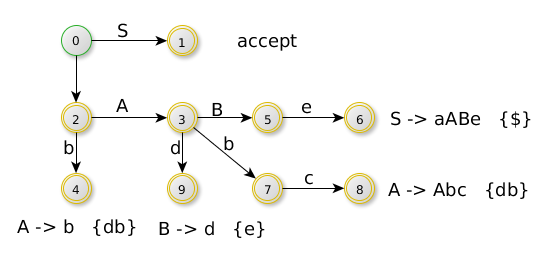
\includegraphics[scale=0.4]{Chapters/Img/c02_14.png}\\
\end{center} 

La sottolineatura significa che se arrivo in questo stato e sto leggendo come prossimo input una d o una b posso fare la riduzione della b usando A. Lo stesso vale per le altre, ovviamente con i loro simboli.
La roba fra parentesi graffe si chiama look-ahead set.

Nel grafo faccio quindi i seguenti passi (i numeri sono i nodi):
\begin{tabular}{ll}
    $0$   &   $abbcde\$$\\
    $0 \rightarrow 2$ consumando \lq $a$ \rq     &  $a || bbcde \$ $\\
    $2 \rightarrow 4$ consumando \lq $b$ \rq     &  $ab || bcde \$ $\\
    4 riduco $A \rightarrow b$  & $aA || bcde$\\
\end{tabular}
A questo punto torno al nodo 2 ovvero il precedente. Vado quindi in 3, perch\'e ho la A al posto della b che avevo prima.\\
torno a 2, vado in 3
\begin{tabular}{ll}
    $3 \rightarrow 7$ consumando \lq $b$ \rq     &  $aAb || cde \$ $\\
    $7 \rightarrow 8$ consumando \lq $c$ \rq     &  $aAbc || de \$ $\\
    8 riduco $A \rightarrow Abc$  & $aA || de$\\
    torno a 7, torno in 3, vado in 9 & \\
    $3 \rightarrow 9$ consumando \lq $d$ \rq     &  $aAd || e \$ $\\
    riduco $B \rightarrow d$ & $aAB || e \$ $\\
    torno a 3, vado in 5, vado in 6 & \\
    $5 \rightarrow 6$ consumando \lq $e$ \rq     &  $aABe || \$ $\\
    6 riduco $S \rightarrow aABe$ & $S || \$ $ \\
    torno a 0, vado in 1, ho finito & \\
\end{tabular}

Noi vogliamo avere grammatiche di tipo LALR(1). Grammatiche: $SLR(1) \subset LALR(1) \subset LR(1)$

\begin{center}
    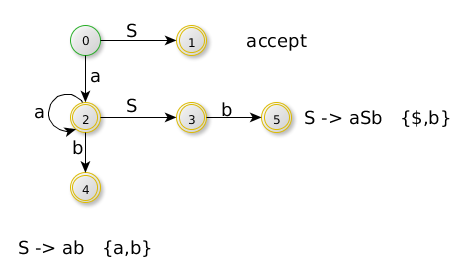
\includegraphics[scale=0.4]{Chapters/Img/c02_15.png}\\
\end{center} 

$S \rightarrow aSb | ab$\\
$w = aaabbb\$$

\begin{tabular}{ll}
    $0$                             &   $aaabbb\$$  \\ 
    $0 \rightarrow 2$               &   $a || aabbb\$$  \\ 
    $2 \rightarrow 2$               &   $aa || abbb\$$  \\ 
    $2 \rightarrow 2$               &   $aaa || bbb\$$  \\ 
    $2 \rightarrow 4$               &   $aaab || bb\$$  \\ 
    4 riduco $S \rightarrow ab$     &    $aaS || bb\$$  \\ 
    torno a 2, vado in 3, vado in 5 & \\
    $3 \rightarrow 5$               &   $aaSb || b\$$  \\ 
    5 riduco $S \rightarrow aSb$    &   $aS || b\$$  \\ 
    torno a 3, vado in 5            & \\
    $3 \rightarrow 5$               &   $aSb || \$$  \\ 
    5 riduco $S \rightarrow aSb$    &   $S || \$$  \\ 
    torno a 0, vado in 1, ho finito & \\
\end{tabular}

Questa \'e una tabella:
\begin{tabular}{|l|l|l|}
    \hline
            &   terminali $\cup \$$                                     &   $V \backslash T$     \\
    \hline
    stati   &   shift-k: leggi un simbolo di input e vai allo stato     &   goto-k: descrive le funzioni di transizione  \\
            &   reduce $A \rightarrow b $                               &   identificate dai non terminali quando consumi roba\\
    \hline
\end{tabular}

\section{Algoritmo di shift/reduce}
(comune a SLR(1), LR(1), LALR(1))

\begin{tabular}{ll}
    input   &   w, tabella di parsing bottom-up di tipo $\diamond$, con $\diamond$ scelto fra $\{SLR(1), LALR(1), LR(1)\}$ G.\\
    output  &   derivazione rightmost di w se $w \in L(G)$, altrimenti error()\\  
\end{tabular}

\begin{lstlisting}
    stack.push(s_0);
    buffer = w$;
    while(true){
        let s = stack.top();
        if(M[s,b] == shift-k){
            stack.push(b);
            stack.push(k);
            let b = buffer.readNext(); 
        } else if(M[s,b] == "reduce A -> beta"){
            stack.pop() 2|beta| simboli;
            let j tale che M[m, A] = gj;
            push(A);
            push(j);
            output "A -> beta";
        } else if(M[s,b] = accetta){
            break;
        } else {
            error();
        }
    }
\end{lstlisting}

*sketo*
$S \rightarrow aSb | ab $

\begin{center}
    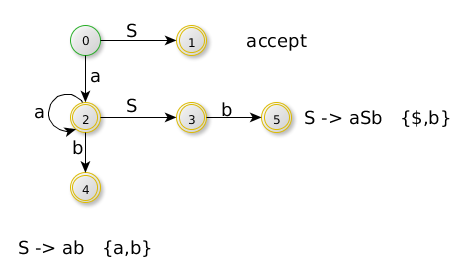
\includegraphics[scale=0.4]{Chapters/Img/c02_15.png}\\
\end{center} 

Questo \'e uguale ma scritto diversamente per separare $\{ \$, b\}$ in $\{4\}$ e $\{b\}$. Nel caso di $w=aaabbb\$$. Una caso rappresenta
il rao pi\'u in alto, mentre l'altro il secondo ramo (pi\'u interno).

\begin{center}
    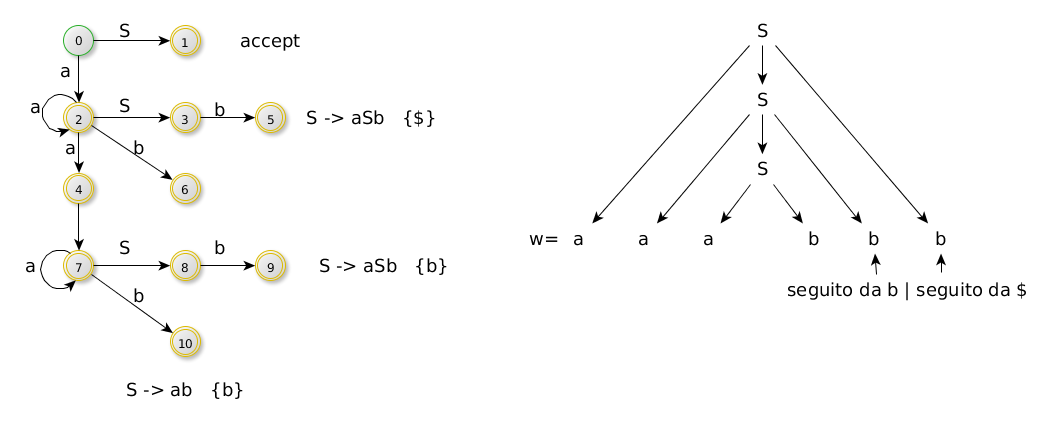
\includegraphics[scale=0.4]{Chapters/Img/c02_16.png}\\
\end{center} 

\begin{itemize}
    \item Automa caratteristico \\
    \item Lookahead Function \\
\end{itemize}

Coppie diverse di questi due insiemi ci danno tipi di grammatiche diverse.

Gli automi che stiamo utilizzando devono essere in grado di ricordare abbastanza da essere in grado di tornare indietro fino al punto 
in cui abbiamo sostituito una certa sequenza di terminali/non terminali con un'altra.

$G = (V,T,S,P)$, aggiungo una produzione $S' \rightarrow S$, $G' = (V \cup \{S'\},T,S',P \cup \{S' \rightarrow S\})$
$A \rightarrow \alpha . \beta $ 

All'inizio ho .S, ovvero non ho ancora letto nulla e devo leggere S.

All'inizio (il nodo iniziale), non ho ancora visto nulla. Visto che S pu\'o iniziare con aSb o ab non sappiamo davanti a quale sviluppo ci troviamo. Il primo stato \'e quindi 

$S' \rightarrow .S$\\
$S \rightarrow .aSb$\\
$S \rightarrow .ab$\\

Questo pu\'o essere visto come un nodo. Da questo stato mi muovo verso un altro stato (con una a-transizione, perch\'e vedo che iniziano 
quasi tutte con a). In questo stato avr\'o:
$S \rightarrow a.Sb$\\
$S \rightarrow a.b$\\

Adesso mi aspetto di vedere l'espansione di una S. Devo quindi aggiungere a questo nodo anche quelle produzioni, e diventa quindi:
$S \rightarrow a.Sb$\\
$S \rightarrow a.b$\\
$S \rightarrow .aSb$\\
$S \rightarrow .ab$\\

Notare che le ultime due sono le stesse delle ultime due del nodo prima. Quella \'e la chiusura, mentre le due prima sono i generatori dello stato (kernel dello stato, \textbf{kernel items}).

Gli stati che sono terminali (ovvero che nol disegno prima avevano le transizioni scritte vicino), sono del tipo $S \rightarrow ab.$ ,
ovvero che hanno incontrato di tutto e di cui si pu\'o eseguire la riduzione. Questi si chiamano \textbf{reducing items}.

Dallo stato con 4 items che avevo prima, si pu\'o fare una b-transizione che va in uno di quelli stati terminali, ovvero:
$S \rightarrow ab.$\\
Questo perch\'e la seconda produzione si aspetta b, che poi completa quello che viene generato da quella produzione.
Sempre da quello stato con 4 produzioni partir\'a anche una a-transizione ed una S-transizione. Per vedere che transizioni devo avere, 
devo vedere la prima lettera dopo il punto per ogni item di quel nodo.

\section{Items}
$G=(V,T,S,P)$\\
$G'=(V \cup \{ S' \},T,S',P \cup \{S' \rightarrow S\})$, con $S' \not\in V$.

Un LR(0)-item di G' \'e una produzione di G con un punto in qualche posizione del body, ovvero $A \rightarrow \alpha . \beta$ .
Alla produzione della forma $A \rightarrow \varepsilon$ corrisponde un solo LR(0)-item, ovvero $A \rightarrow . $\\
L'item $A \rightarrow \alpha . \beta $ \'e detto:
\begin{tabular}{ll}
    iniziale    &   se $A = S' \land \alpha = \varepsilon \land \beta = S$, cio\'e se l'item \'e $S' \rightarrow .S$\\
    accepting   &   se $A = S' \land \alpha = S \land \beta = \varepsilon $, cio\'e se l'item \'e $S' \rightarrow S.$\\
    kernel      &   se \'e un iniziale o tale che $\alpha != \varepsilon$ \\
    closure     &   se $\alpha = \varepsilon$ e non \'e iniziale \\
    reducing    &   se non \'e accepting e $\beta = \varepsilon$, cio\'e se il punto \'e in fondo $\land !accepting$ \\
\end{tabular}
